\documentclass[a4paper,landscape]{article}
\usepackage[margin=1cm]{geometry}
\usepackage{tikz}
\usetikzlibrary{shapes.geometric}

\pagestyle{empty}

\begin{document}

\begin{center}
    {\Huge \bfseries \sffamily Guitalele Fretboard Note Map}\\[0.2cm]
    {\Large \sffamily Tuning: G--D--G--B--D--G (Low to High)}\\[0.6cm]
\end{center}

\noindent
\centering
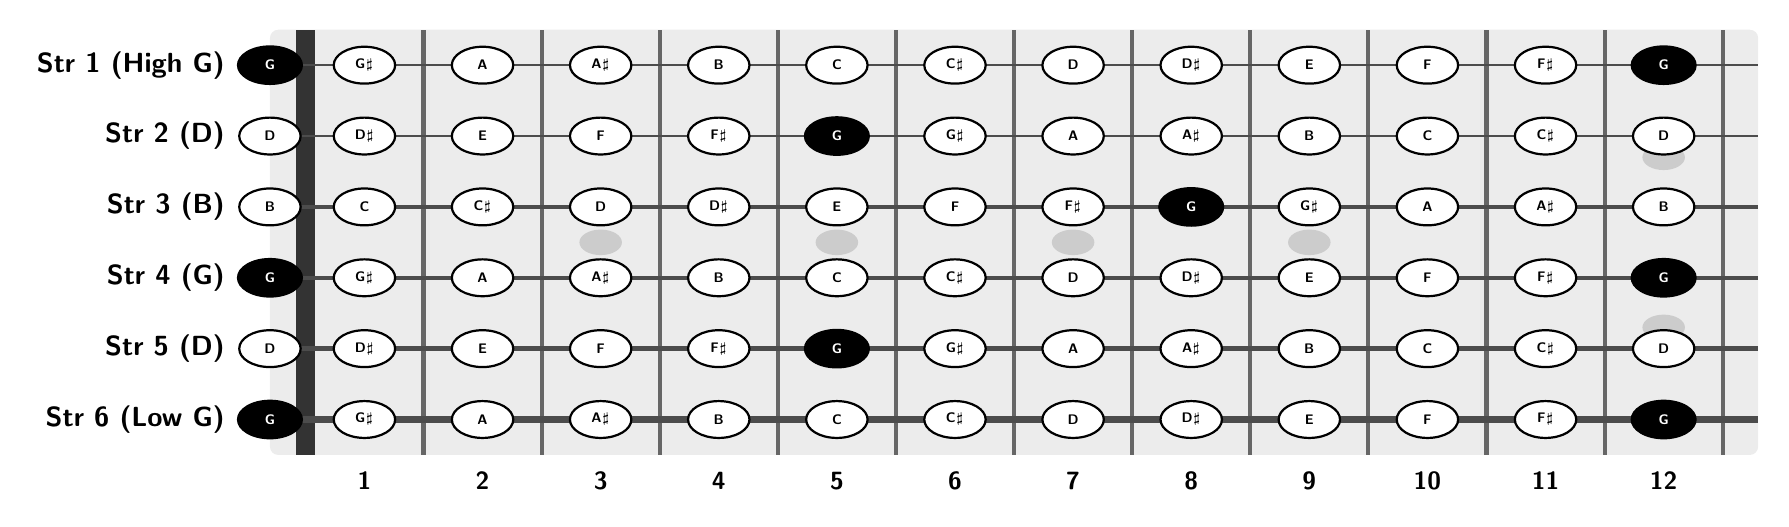
\begin{tikzpicture}[xscale=1.5, yscale=0.9]

    % Fretboard parameters
    % X: Frets 0 (Nut) to 12
    % Y: Strings 1 (Top / High G) to 6 (Bottom / Low G)

    % Fretboard wood background
    \fill[gray!15, rounded corners=3pt] (-0.3, 0.5) rectangle (12.3, 6.5);

    % Nut (Fret 0)
    \fill[black!80] (-0.08, 0.5) rectangle (0.08, 6.5);

    % Draw Frets (1 to 12)
    \foreach \fret in {1,...,12} {
        \draw[line width=1.5pt, black!60] (\fret, 0.5) -- (\fret, 6.5);
        \node[below, font=\sffamily\bfseries\small] at (\fret - 0.5, 0.4) {\fret};
    }

    % Fretboard Inlay Markers (3, 5, 7, 9 = Single Dot, 12 = Double Dot)
    \foreach \fret in {3, 5, 7, 9} {
        \fill[gray!40] (\fret - 0.5, 3.5) circle (0.18cm);
    }
    % 12th Fret Double Dot
    \fill[gray!40] (11.5, 2.3) circle (0.18cm);
    \fill[gray!40] (11.5, 4.7) circle (0.18cm);

    % Draw Strings (6 at bottom, 1 at top)
    \foreach \str/\thickness in {1/0.8pt, 2/1.0pt, 3/1.2pt, 4/1.5pt, 5/1.8pt, 6/2.2pt} {
        \draw[line width=\thickness, black!70] (-0.5, 7 - \str) -- (12.3, 7 - \str);
    }

    % String Labels (Left Side)
    \node[left, font=\sffamily\bfseries] at (-0.6, 6) {Str 1 (High G)};
    \node[left, font=\sffamily\bfseries] at (-0.6, 5) {Str 2 (D)};
    \node[left, font=\sffamily\bfseries] at (-0.6, 4) {Str 3 (B)};
    \node[left, font=\sffamily\bfseries] at (-0.6, 3) {Str 4 (G)};
    \node[left, font=\sffamily\bfseries] at (-0.6, 2) {Str 5 (D)};
    \node[left, font=\sffamily\bfseries] at (-0.6, 1) {Str 6 (Low G)};

    % -------------------------------------------------------------
    % PLACING NOTES (String, Fret, Note Name, IsRoot)
    % Y-coordinate = 7 - String Number
    % X-coordinate = Fret - 0.5 (Open = -0.3)
    % -------------------------------------------------------------

    \newcommand{\note}[4]{
        % #1: String (1-6), #2: Fret (0-12), #3: Note Name, #4: IsRoot (1 or 0)
        \ifnum#2=0
            \def\xpos{-0.3}
        \else
            \pgfmathsetmacro{\xpos}{#2 - 0.5}
        \fi
        \pgfmathsetmacro{\ypos}{7 - #1}

        \ifnum#4=1
            % Root Notes (G) highlighted in dark gray/black fill with white text
            \fill[black] (\xpos, \ypos) circle (0.28cm);
            \node[white, font=\sffamily\bfseries\tiny] at (\xpos, \ypos) {#3};
        \else
            % Regular Notes in white circle with black text
            \fill[white, draw=black, line width=0.8pt] (\xpos, \ypos) circle (0.26cm);
            \node[black, font=\sffamily\bfseries\tiny] at (\xpos, \ypos) {#3};
        \fi
    }

    % String 1 (High G)
    \note{1}{0}{G}{1} \note{1}{1}{G$\sharp$}{0} \note{1}{2}{A}{0} \note{1}{3}{A$\sharp$}{0}
    \note{1}{4}{B}{0} \note{1}{5}{C}{0} \note{1}{6}{C$\sharp$}{0} \note{1}{7}{D}{0}
    \note{1}{8}{D$\sharp$}{0} \note{1}{9}{E}{0} \note{1}{10}{F}{0} \note{1}{11}{F$\sharp$}{0} \note{1}{12}{G}{1}

    % String 2 (D)
    \note{2}{0}{D}{0} \note{2}{1}{D$\sharp$}{0} \note{2}{2}{E}{0} \note{2}{3}{F}{0}
    \note{2}{4}{F$\sharp$}{0} \note{2}{5}{G}{1} \note{2}{6}{G$\sharp$}{0} \note{2}{7}{A}{0}
    \note{2}{8}{A$\sharp$}{0} \note{2}{9}{B}{0} \note{2}{10}{C}{0} \note{2}{11}{C$\sharp$}{0} \note{2}{12}{D}{0}

    % String 3 (B)
    \note{3}{0}{B}{0} \note{3}{1}{C}{0} \note{3}{3}{D}{0} \note{3}{2}{C$\sharp$}{0}
    \note{3}{4}{D$\sharp$}{0} \note{3}{5}{E}{0} \note{3}{6}{F}{0} \note{3}{7}{F$\sharp$}{0}
    \note{3}{8}{G}{1} \note{3}{9}{G$\sharp$}{0} \note{3}{10}{A}{0} \note{3}{11}{A$\sharp$}{0} \note{3}{12}{B}{0}

    % String 4 (G)
    \note{4}{0}{G}{1} \note{4}{1}{G$\sharp$}{0} \note{4}{2}{A}{0} \note{4}{3}{A$\sharp$}{0}
    \note{4}{4}{B}{0} \note{4}{5}{C}{0} \note{4}{6}{C$\sharp$}{0} \note{4}{7}{D}{0}
    \note{4}{8}{D$\sharp$}{0} \note{4}{9}{E}{0} \note{4}{10}{F}{0} \note{4}{11}{F$\sharp$}{0} \note{4}{12}{G}{1}

    % String 5 (D)
    \note{5}{0}{D}{0} \note{5}{1}{D$\sharp$}{0} \note{5}{2}{E}{0} \note{5}{3}{F}{0}
    \note{5}{4}{F$\sharp$}{0} \note{5}{5}{G}{1} \note{5}{6}{G$\sharp$}{0} \note{5}{7}{A}{0}
    \note{5}{8}{A$\sharp$}{0} \note{5}{9}{B}{0} \note{5}{10}{C}{0} \note{5}{11}{C$\sharp$}{0} \note{5}{12}{D}{0}

    % String 6 (Low G)
    \note{6}{0}{G}{1} \note{6}{1}{G$\sharp$}{0} \note{6}{2}{A}{0} \note{6}{3}{A$\sharp$}{0} \note{6}{4}{B}{0} \note{6}{5}{C}{0} \note{6}{6}{C$\sharp$}{0} \note{6}{7}{D}{0}
    \note{6}{8}{D$\sharp$}{0} \note{6}{9}{E}{0} \note{6}{10}{F}{0} \note{6}{11}{F$\sharp$}{0} \note{6}{12}{G}{1}

\end{tikzpicture}

\vspace{0.5cm}
\begin{center}
    \small\sffamily
    \textbf{Legend:} \textbf{Black circles} indicate Root notes (\textbf{G}). 
    \textbf{White circles} indicate chord/scale intervals across the fretboard.
\end{center}

\end{document}
